\part{Solutions-to-DEs}
\lecture{Solutions to DEs}{Solutions-to-DEs}
\section{Solutions to DEs}

\title{Ordinary Differential Equations}
\subtitle{Math 232 - Week 1, Day 2}
\date{29 Aug 2012}

\begin{frame}
  \titlepage
\end{frame}

\begin{frame}
  \frametitle{Outline}
  \tableofcontents[pausesection,hideothersubsections]
\end{frame}


\subsection{Solutions to DEs}


\begin{frame}
  \frametitle{What is a solution to a DE?}

  \begin{eqnarray*}
    y' & = & y
  \end{eqnarray*}

   \uncover<2->{
     Solution: $y=3e^t$
   }

  \uncover<3->{

    How do you check? 
    \begin{itemize}
    \item Substitute into the left hand side.
    \item Substitute into the right hand side.
    \item See if they are the same.
    \end{itemize}

  }

  \uncover<4->{
    Check: 
    \begin{eqnarray*}
      y' & = & 3e^t \\
      y  & = & 3e^t
    \end{eqnarray*}

    The same!
  }

\end{frame}


\begin{frame}
  \frametitle{What is a solution to a DE?}

  \begin{eqnarray*}
    y' & = & y
  \end{eqnarray*}

  Solution: $y=2e^t$

  \uncover<2->{
    Check: 
    \begin{eqnarray*}
      y' & = & 2e^t \\
      y  & = & 2e^t
    \end{eqnarray*}

    The same!
  }


\end{frame}


\begin{frame}
  \frametitle{What is a solution to a DE?}

  \begin{eqnarray*}
    y' & = & y, \\
    y(0) & = & 4
  \end{eqnarray*}

  Neither is a solution! 

  \uncover<2->{
    Solution: $y=4e^t$

    Check: 
    \begin{eqnarray*}
      y' & = & 4e^t \\
      y  & = & 4e^t \\
      y(0) & = & 4
    \end{eqnarray*}

    This is \textbf{the} solution.
  }

\end{frame}


\begin{frame}
  \frametitle{What is a solution to a DE?}

  Show that 
  \begin{eqnarray*}
    y & = & 3 e^{2t} - \half
  \end{eqnarray*}
  is a solution to
  \begin{eqnarray*}
    y' & = & 2y + 1.
  \end{eqnarray*}

  \uncover<2->{
    \begin{eqnarray*}
      y' & = & 6 e^{2t} \\
      2y+1 & = & 2(3 e^{2t} - \half) +1 \\
      & = & 6 e^{2t}
    \end{eqnarray*}
  }


\end{frame}


\begin{frame}
  \frametitle{What is a solution to a DE?}

  Show that 
  \begin{eqnarray*}
    y & = & \half e^{2t} - \half
  \end{eqnarray*}
  is a solution to
  \begin{eqnarray*}
    y' & = & 2y + 1, \\
    y(0) & = & 0.
  \end{eqnarray*}

  \uncover<2->{
    \begin{eqnarray*}
      y' & = & e^{2t} \\
      2y+1 & = & 2\lp\half e^{2t} - \half\rp +1 \\
      & = & e^{2t} \\
      y(0) & = & \half e^0 - \half \\
      & = & 0
    \end{eqnarray*}
  }



\end{frame}


\subsection{Slope Fields}

\begin{frame}
  \frametitle{What is the derivative?}

  The derivative is the slope of the tangent line.

  \begin{tabular}{lll}
    if y'=2 & slope=2 & (inc) \\
    if y'=3 & slope=3 & (inc) \\
    if y'=-2 & slope=-2 & (dec) \\
  \end{tabular}


\end{frame}


\begin{frame}
  \frametitle{Example}

  \begin{eqnarray*}
    y' & = & 5t + 3, \\
    \int y' ~ dt & = & \int 5t + 3 ~ dt \\
    \uncover<2->{y & = & \frac{5}{2} t^2 + 3t + C}
  \end{eqnarray*}

  \uncover<2->{We get a ``family of solutions.'' }

  \uncover<3->{
    If $y(0)=2$ then
    \begin{eqnarray*}
      y(0) & = & \frac{5}{2} (0)^2 + 3(0) + C, \\
      2    & = & C
    \end{eqnarray*}
  }


\end{frame}


\begin{frame}
  \frametitle{Slope Fields}

  Given the differential equation can we predict the \textit{general
    behavior} of the solution? (Qualitative behavior)

  If we have 
  \begin{eqnarray*}
    y' & = & f(t,y),
  \end{eqnarray*}
  then if we know that the function goes through a point, $t=a$ and
  $y(a)=v$, then we can calculate the slope of the tangent line.

\end{frame}


\begin{frame}
  \frametitle{Slope Fields}

  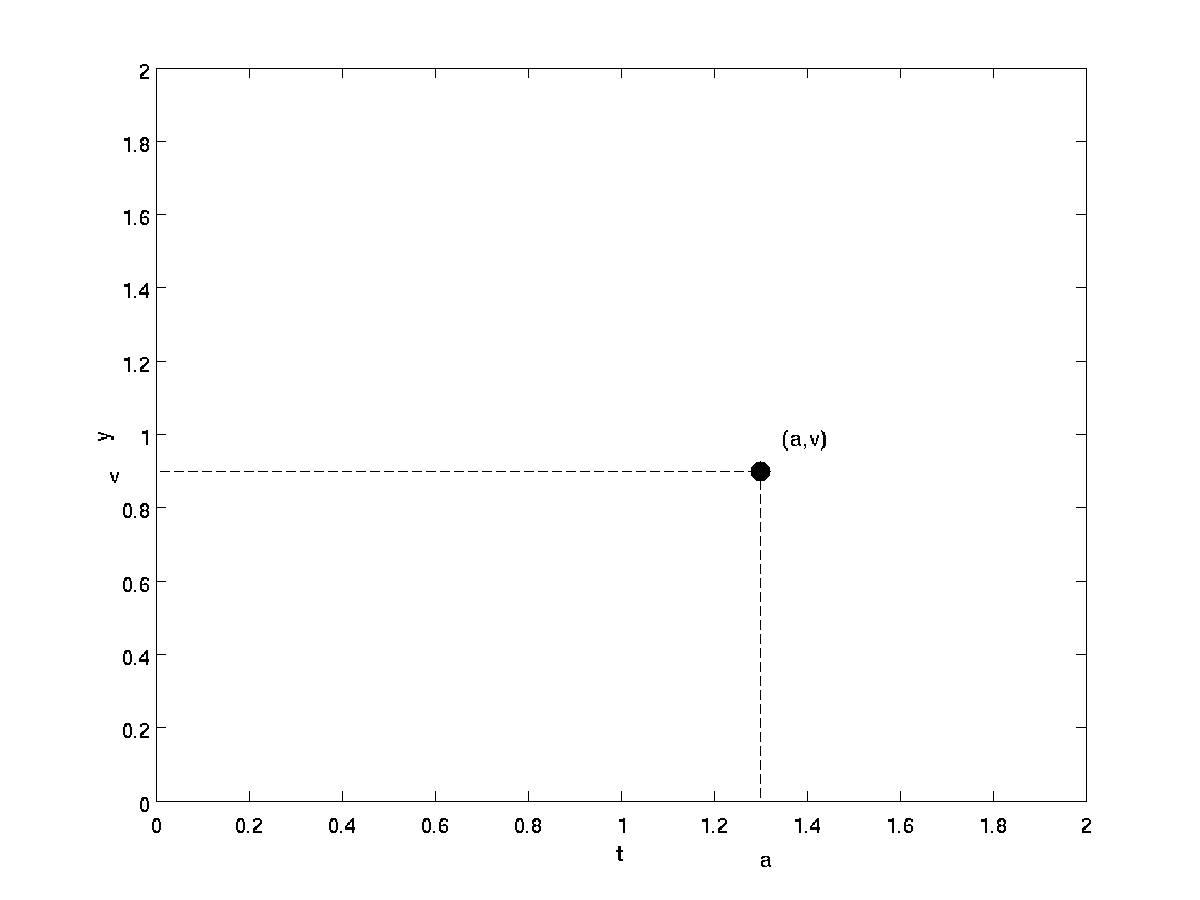
\includegraphics[height=8cm]{img/singlePointInSlopeField}

\end{frame}


\begin{frame}
  \frametitle{Slope Fields}

  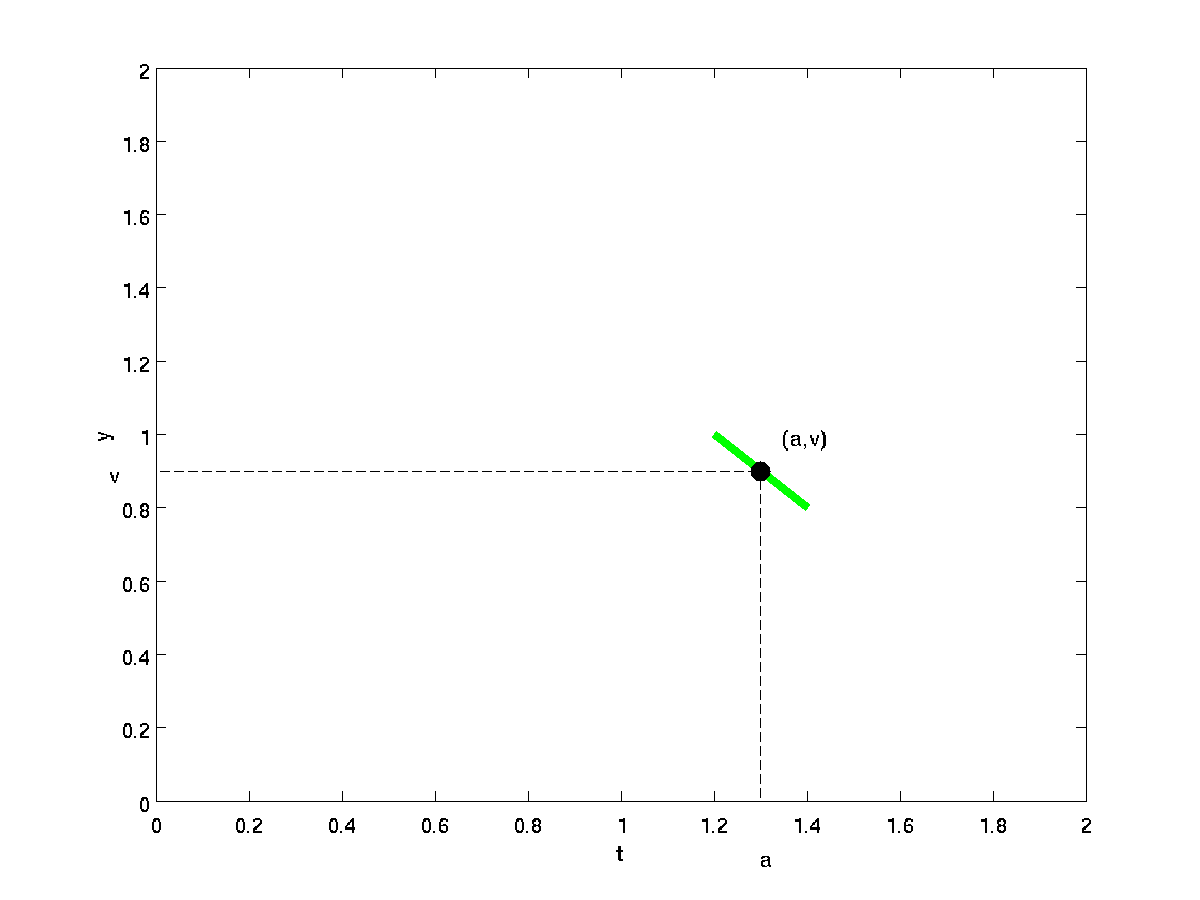
\includegraphics[height=8cm]{img/singlePointWithSlopeField}

\end{frame}


\begin{frame}
  \frametitle{Example}

  \vspace*{-4em}

  \begin{eqnarray*}
    y' & = & 2y
  \end{eqnarray*}

  At $t=3$ if you happen to know that $y=4$ then the slope is 2(4)=8.

  At $t=3$ if you happen to know that $y=5$ then the slope is 2(5)=10.

  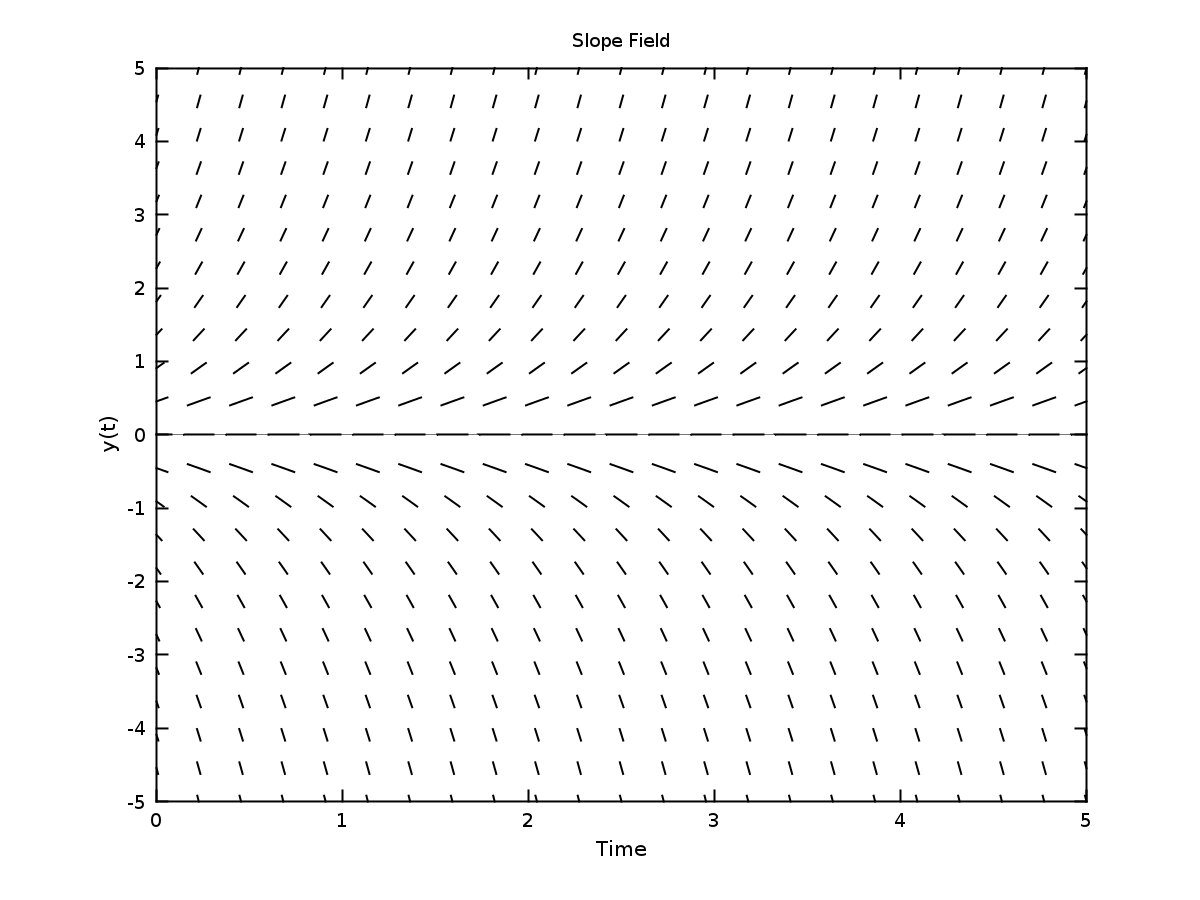
\includegraphics[height=4cm]{img/week1Day2SlopeField}

  A direction field is a collection of segments that indicate the
  tangent lines. 
  
\end{frame}


\begin{frame}
  \frametitle{Example}

  \vspace*{-4em}

  \begin{eqnarray*}
    y' & = & y - t
  \end{eqnarray*}

  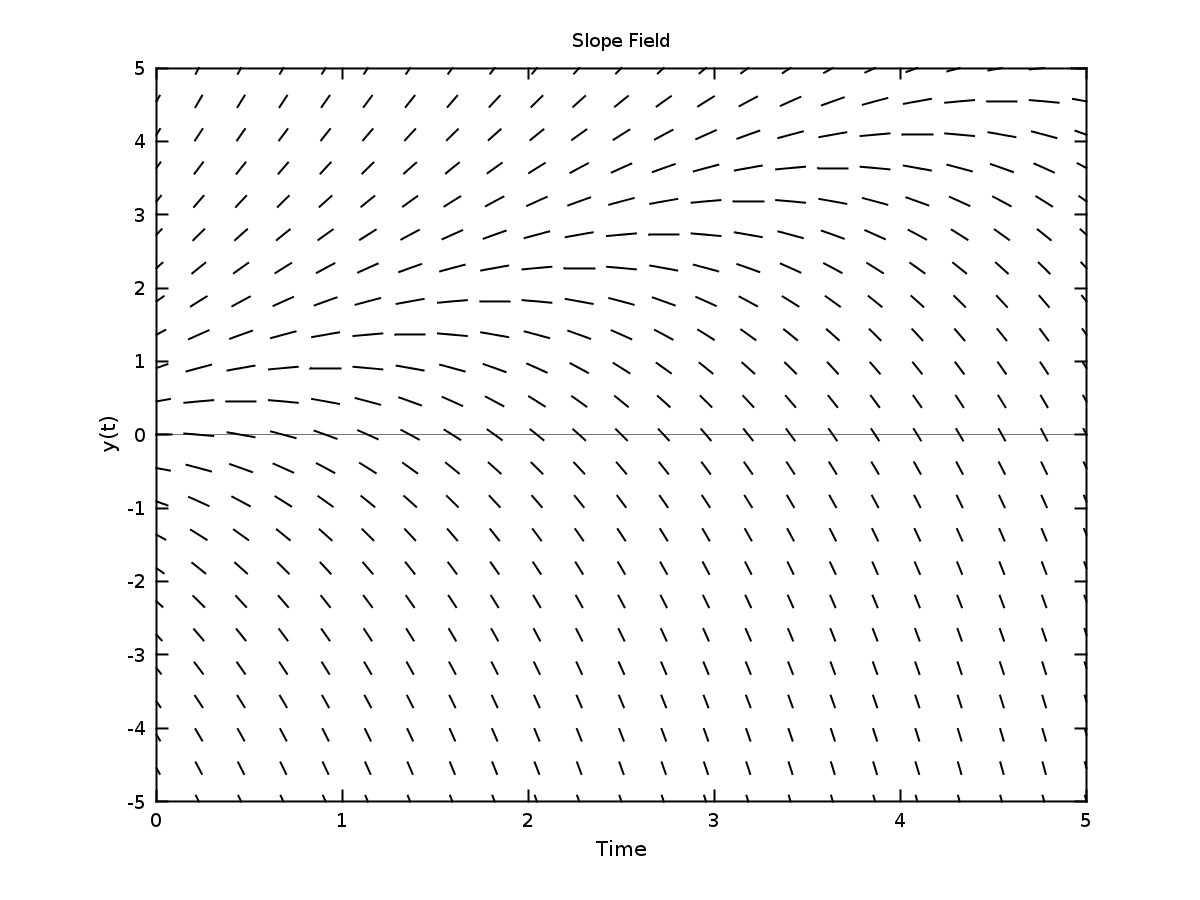
\includegraphics[height=5cm]{img/week1Day2SlopeField2}

  Tools:
  \begin{itemize}
  \item A ``stationary point'' is a point where $y'=0$.
  \item An isocline is a curve where $y'$ is equal to a constant.
  \end{itemize}

\end{frame}


\begin{frame}
  \frametitle{Example}

  \vspace*{-4em}

  \begin{eqnarray*}
    y' & = & y^2 - 3y
  \end{eqnarray*}

  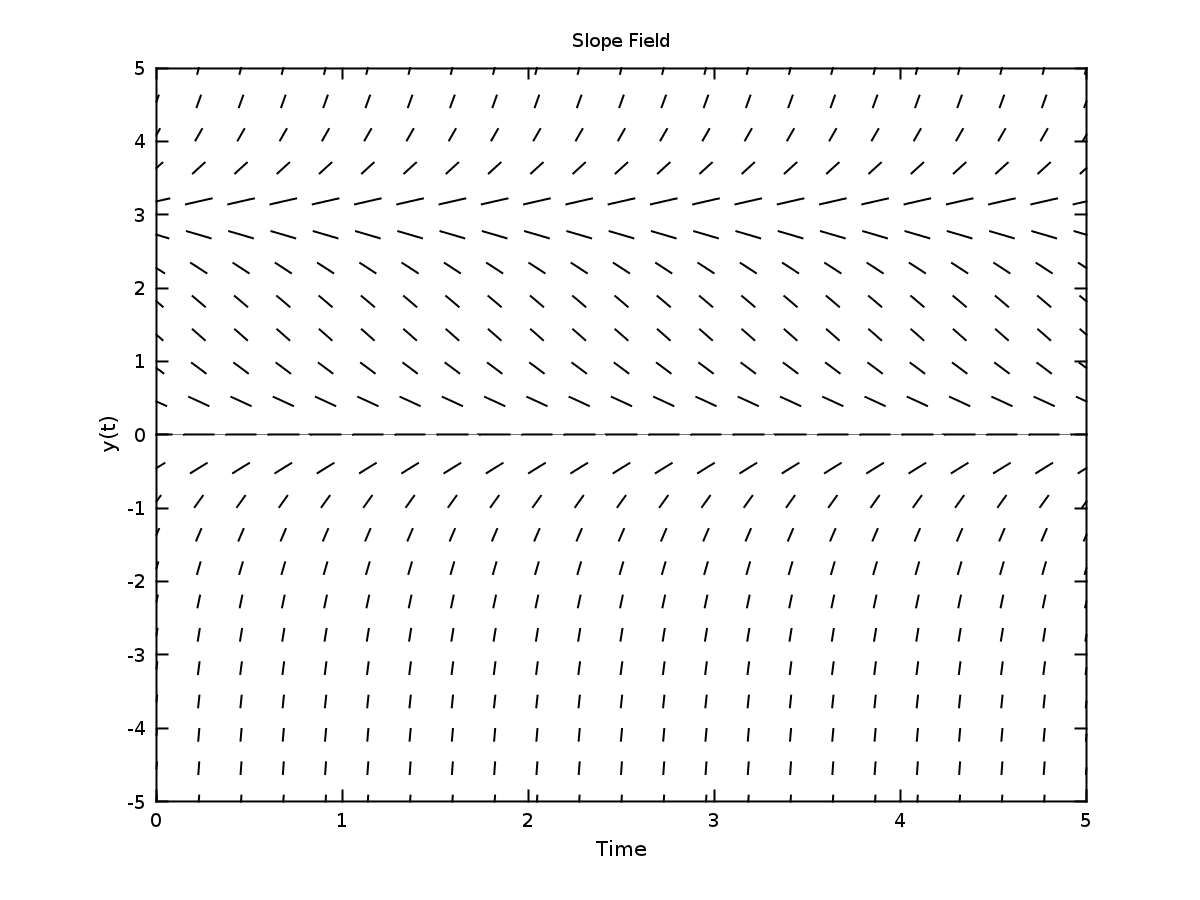
\includegraphics[height=5cm]{img/week1Day2SlopeField3}

  Definition: An equilibrium solution is a value for which the
  solution does not change in time.

  \uncover<2->{$y(t)=0$ and $y(t)=3$ are equilibrium solutions.}

\end{frame}

\subsection{Stability}

\begin{frame}
  \frametitle{Stability}

  \begin{itemize}
  \item An \textit{equilibrium solution} is \textbf{stable} if values
    of the solution tend to stay close to it as $t$ increases.
  \item An \textit{equilibrium solution} is \textbf{unstable} if
    values of the solution tend to move away from it as $t$ increases.
  \end{itemize}

  In the previous example $y=0$ is stable while $y=3$ is unstable.

\end{frame}



% LocalWords:  Clarkson pausesection hideothersubsections isocline DEs
